\documentclass[11pt,a4paper]{article}
\usepackage[utf8]{inputenc}
\usepackage[french]{babel}
\usepackage[T1]{fontenc}
\usepackage{amsmath}
\usepackage{amsfonts}
\usepackage{amssymb}
\usepackage{makeidx}
\usepackage{graphicx}

\usepackage{tcolorbox}

\usepackage{lmodern}
\usepackage{fourier}
\usepackage[left=2cm,right=2cm,top=2cm,bottom=2cm]{geometry}
\author{AMONA Birewa Audrey}
\title{ Tp 06 Sécurité et site administration }
\begin{document}
\maketitle
\tableofcontents
\begin{abstract}
Ce TP contient 3 parties indépendantes. D’abord nous nous pencherons sur l’authentification. En-
suite nous explorerons les problèmes de sécurité : CSRF, HTTPS, clé de chiffrement et détournement
de clic. Enfin nous verrons comment customiser le site d’administration.
\end{abstract}
\section{Authentification}
\begin{enumerate}
\item Dans le Tp précédent, nous avions spécifié les différentes fonctionnalités en fonction des utilisateurs du système:
\begin{center}
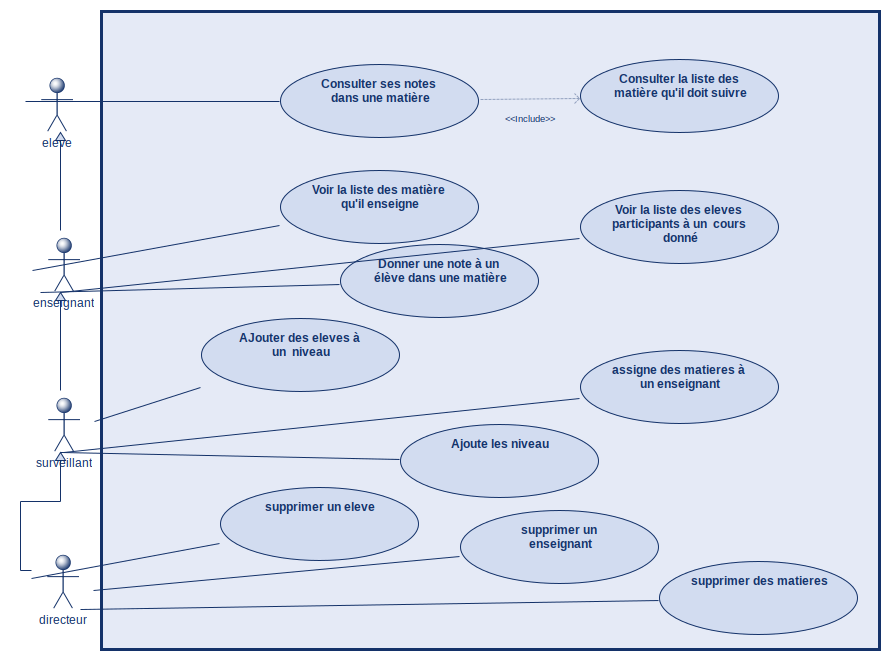
\includegraphics[scale=0.4]{images/cas.png}
\end{center}
Il étais convenu que seul les enseignant, les surveillants ou encore le directeur peuvent avoir accès au formulaire d'ajout de note.
\item Dans le site administration, nous remarquons qu'il y'a deux modèles de plus \textbf{ Users} et \textbf{Groups}, que nous n'avons pas ajouté nous même. Le modèle \textbf{Users} possède les attributs suivant: username, lastname, firstname, email adress, staff, status. Ilpossède un enregistrement qui a pour username le nom de notre superutilisateur créé.

\item Nous allons créer des groupes avec les différents roles du diagramme de cas d'utilisation précédent.
\begin{center}
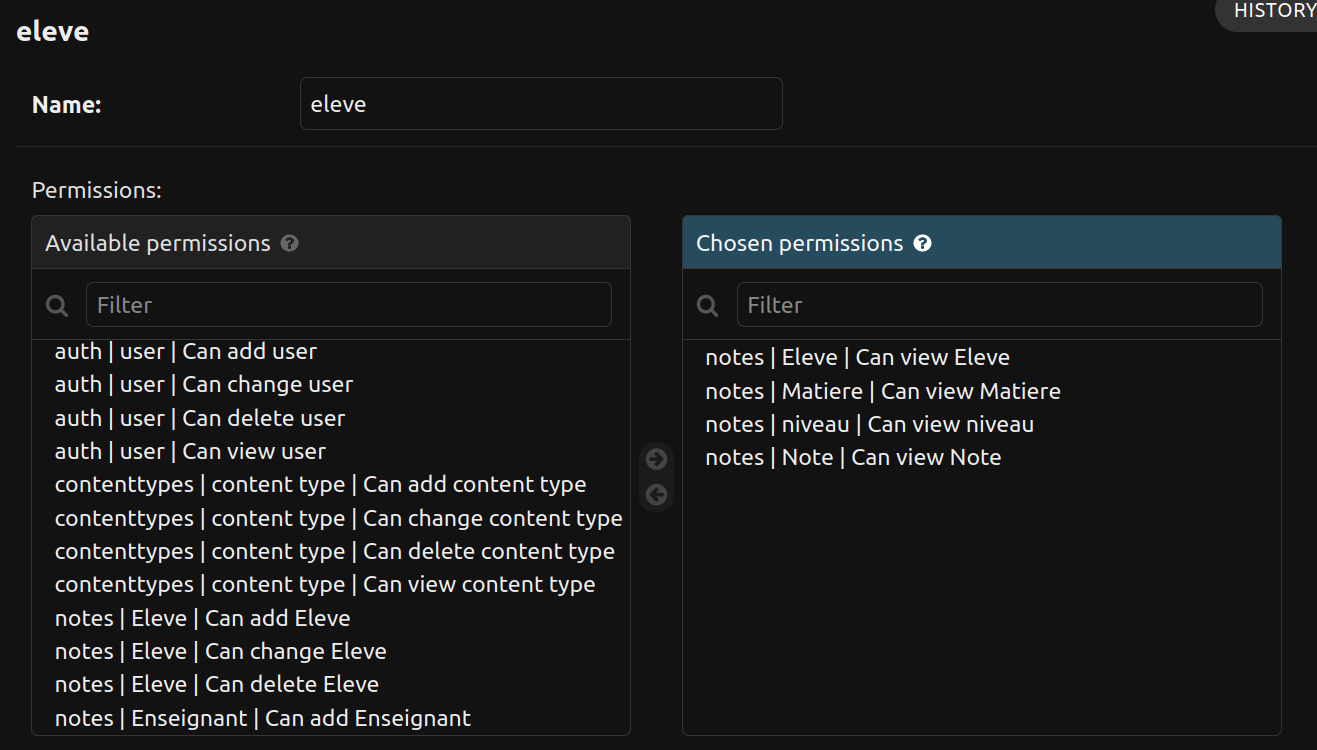
\includegraphics[scale=0.3]{images/1.png}
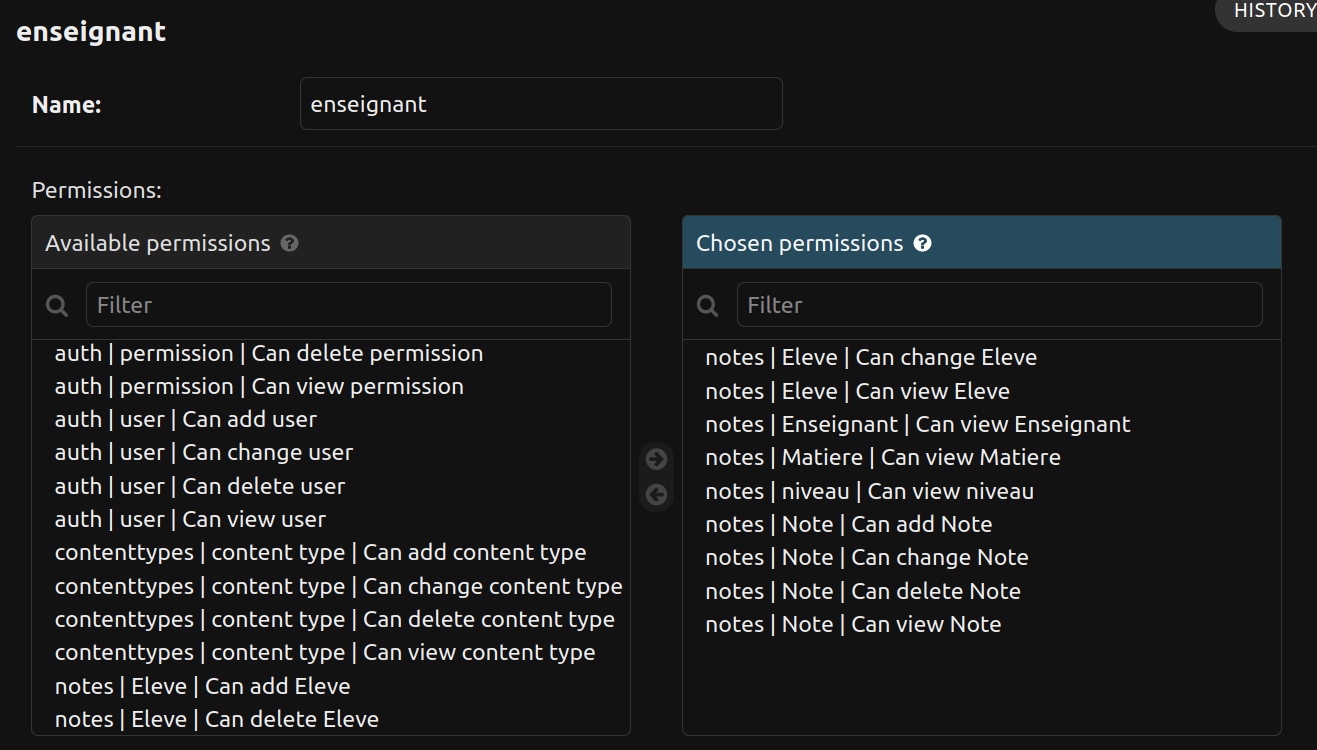
\includegraphics[scale=0.3]{images/2.png}
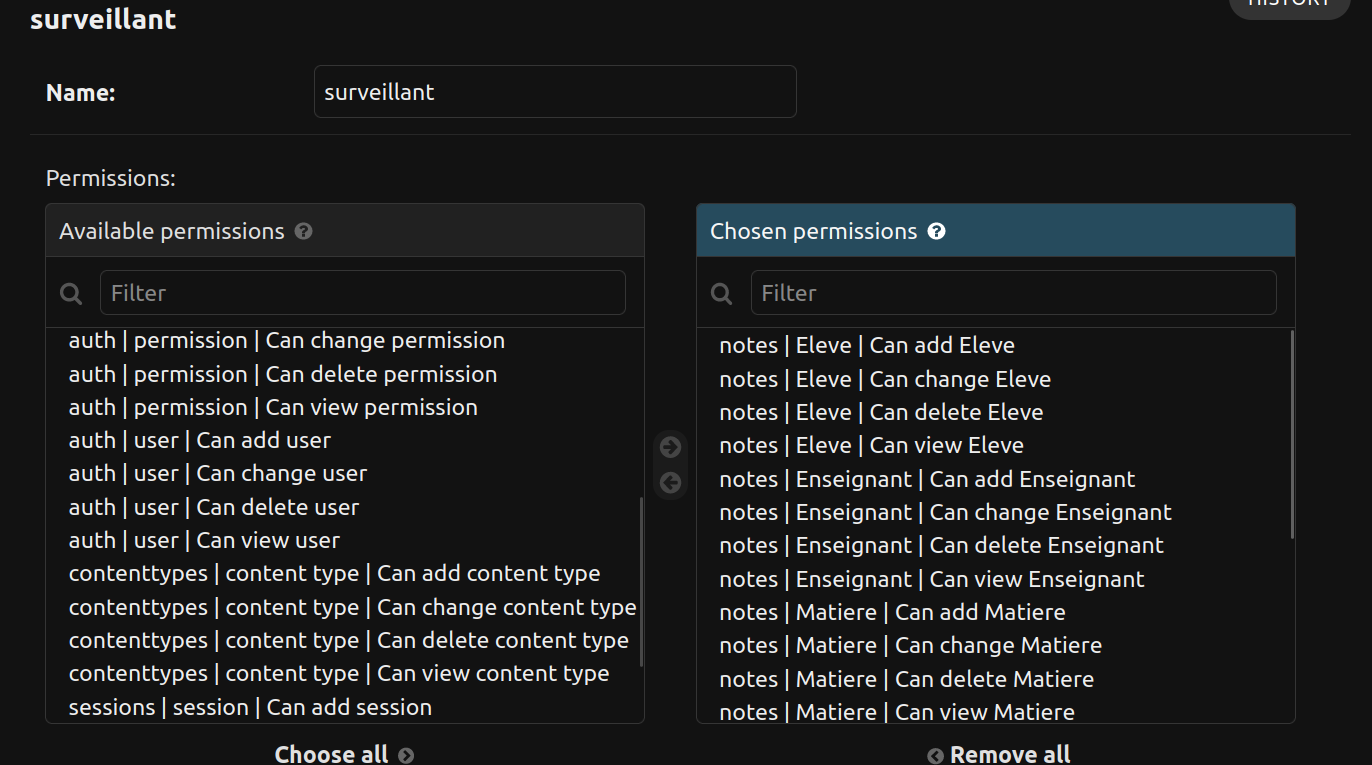
\includegraphics[scale=0.3]{images/3.png}
\end{center}
\item Django fournit une classe User qui contient l’ensemble des informations nécessaires à l’authentification
et aux autorisations Nous pouvons étendre ce modèle sans modifier nos modèles utilisateurs par défaut soit:
	\begin{itemize}
		\item En créant une relation d'héritage entre notre modèle et le modèle par défaut \textbf{Users}
		\item En créant une relation OneToOne entre notre modèle et le modèle par défaut \textbf{Users}
	\end{itemize}
\item Nous allons procéder à la création OneToOne entre les deux modèles, lorsqu'on lance \textbf{py manage.py makemigrations}, on a l'erreur suivante:
\begin{center}
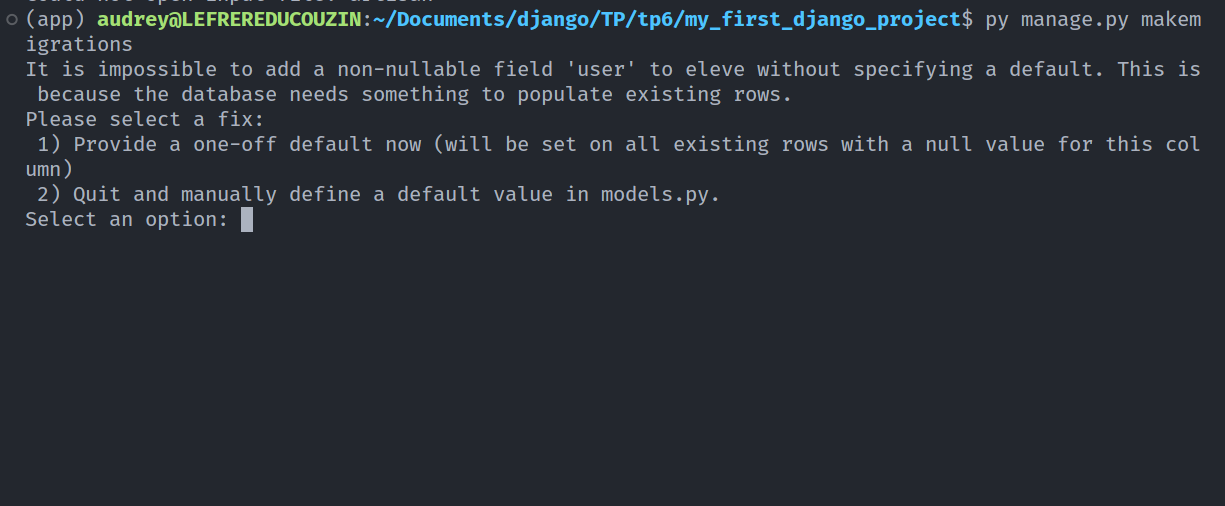
\includegraphics[scale=0.3]{images/error.png}
\end{center}
Ensuite on corrige le modèle en rendant l'attribut \textbf{user} nullable:
\begin{center}
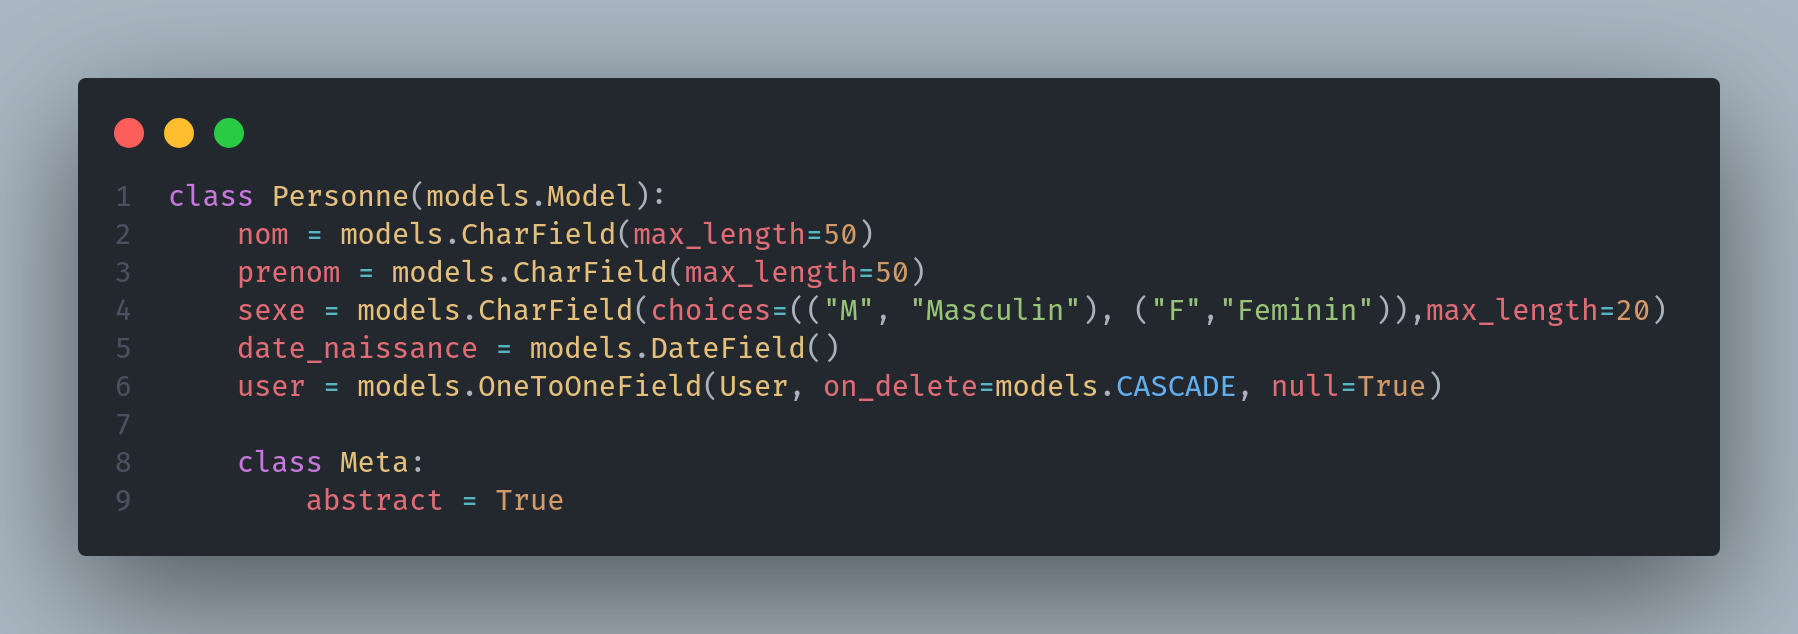
\includegraphics[scale=0.2]{images/per.png}
\end{center}
\item Nous allons maintenant créer une instance de \textbf{User} pour chaque personne que nous avions créé:

\begin{center}
	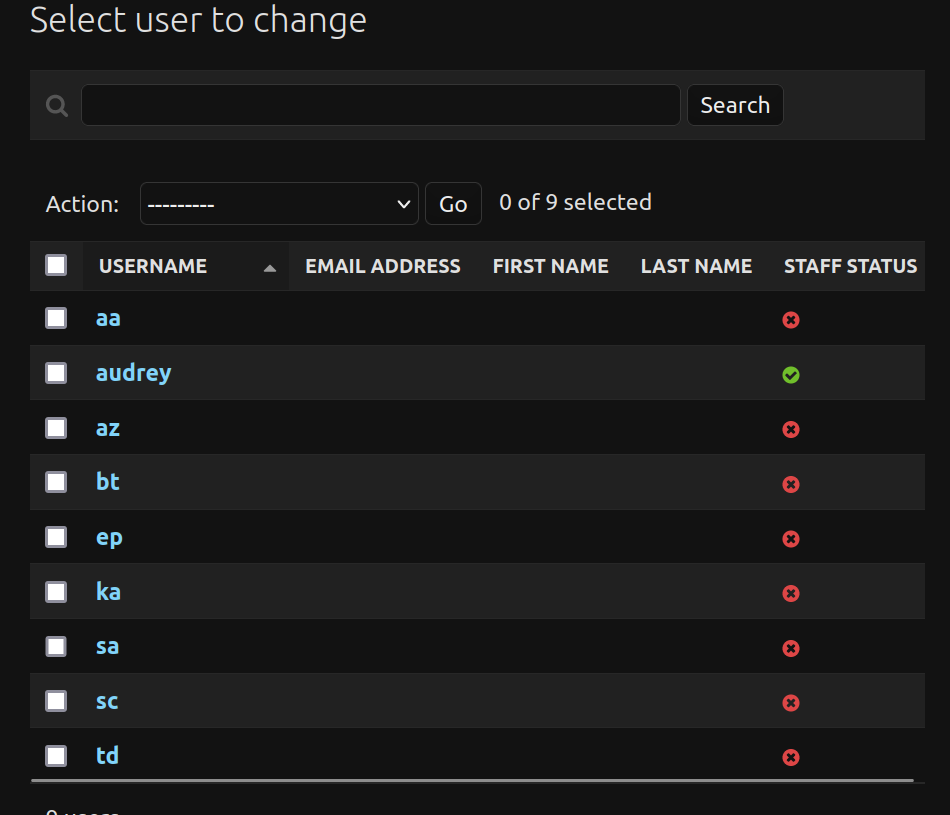
\includegraphics[scale=0.3]{images/users.png}
\end{center}
\item Nous allons maintenant enlever la propriété nullable sur l'attribut précédemment ajouter. Losqu'on essaie de relancer les migration, on a le message suivant au terminal:
\begin{center}
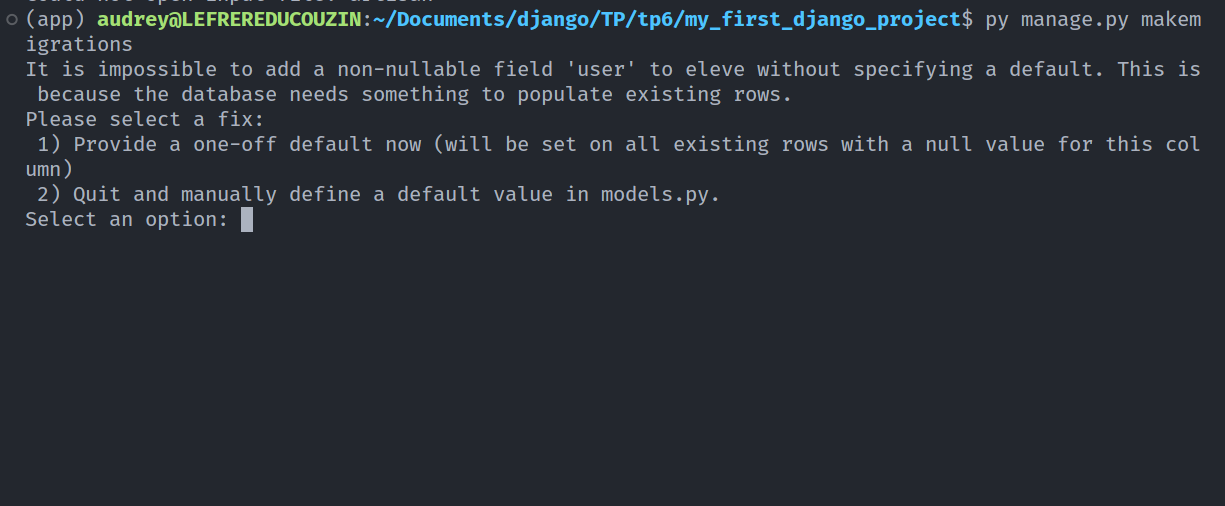
\includegraphics[scale=0.3]{images/error.png}
\end{center}
\end{enumerate}
\end{document}